% ICASSP 2027 working manuscript. Final author names and affiliations are required.
\documentclass{article}
\usepackage{spconf,amsmath,graphicx,booktabs,tikz}
\usepackage[hidelinks]{hyperref}
\usetikzlibrary{arrows.meta,positioning,fit,calc,backgrounds}

% Keep float-only pages compact: place wide tables and figures at the top,
% with any unavoidable slack collected at the page bottom.
\makeatletter
\setlength{\@fptop}{0pt}
\setlength{\@fpsep}{12pt}
\setlength{\@fpbot}{0pt plus 1fil}
\setlength{\@dblfptop}{0pt}
\setlength{\@dblfpsep}{12pt}
\setlength{\@dblfpbot}{0pt plus 1fil}
\makeatother
\renewcommand{\topfraction}{0.95}
\renewcommand{\bottomfraction}{0.95}
\renewcommand{\textfraction}{0.06}
\renewcommand{\floatpagefraction}{0.80}
\renewcommand{\dbltopfraction}{0.95}
\renewcommand{\dblfloatpagefraction}{0.80}
\setlength{\textfloatsep}{12pt plus 2pt minus 2pt}
\setlength{\floatsep}{10pt plus 2pt minus 2pt}
\setlength{\intextsep}{10pt plus 2pt minus 2pt}

\def\x{{\mathbf x}}
\def\L{{\cal L}}

\title{Spatial and Frequency Fusion with Normal References for Long-Tailed Weld Defect Detection}

\name{\shortstack{Guanwei Lu$^{1}$ \qquad Zilai Wang$^{2}$ \qquad Huwenkang Zhang$^{3}$\\
Gang Luo$^{4,*}$ \qquad Zhengji Liu$^{5,*}$}\thanks{*Corresponding authors: Gang Luo (hi.gangluo@gmail.com) and Zhengji Liu (21062388r@connect.polyu.hk).}}
\address{$^{1}$College of Mechatronics and Control Engineering, Shenzhen University,  Guangdong Province, China\\
$^{2}$School of Computer Science and Engineering,\\South China University of Technology, Guangdong Province, China\\
$^{3}$Aberdeen Institute of Data Science and Artificial Intelligence,\\South China Normal University, Guangdong Province, China\\
$^{4}$Shenzhen Pingze Intelligent Technology Co., Ltd., Guangdong Province, China\\
$^{5}$School of Optometry, The Hong Kong Polytechnic University, Hong Kong SAR, China}

\begin{document}
\ninept
\maketitle

\begin{abstract}
Long-tailed object detection suffers from missed detections and class confusion in rare classes with limited training samples. Class confidence alone can struggle to distinguish underrepresented objects from background variations, motivating structural evidence beyond class predictions. We propose NORA, which uses normal references to fuse spatial and frequency evidence for candidate re-evaluation. NORA measures transitions across candidate interiors, boundaries, and surrounding regions, normalizes them against comparable normal-region statistics, and combines the two branches using uncertainty and anomaly strength. On an industrial annular weld validation set, candidate re-evaluation reduces the miss rate from 21.2\% to 9.1\% and the misclassification rate from 63.6\% to 51.5\% on the evaluated rare-defect subset. The class-aware matched rate across all classes increases from 86.48\% to 92.53\%. These results demonstrate the value of normal-reference evidence for rare-defect detection under class imbalance.
\end{abstract}

\begin{keywords}
Long-tailed defect detection, annular weld inspection, spatial--frequency fusion, normal-reference conditioning, candidate reliability.
\end{keywords}

\section{Introduction}

Automated visual inspection is essential for weld-quality control in high-throughput manufacturing. Annular welds are especially challenging because the seam is a closed, periodically repeating structure, whereas reflectance, width, and illumination vary around the circumference. Operationally important defects can be rare, weak, or incomplete. A detector may consequently assign a low score to a true tail defect for the same visual reason that it assigns a low score to a normal local variation. Once a fixed threshold removes the candidate, downstream classification cannot recover it.

Long-tailed detection has mainly addressed imbalance through training schedules, additional supervision, or classifier adjustment. SimLTD transfers head-class knowledge to tail classes through staged training~\cite{tran2025simltd}. RichSem introduces image-level semantics and coarse locations as supplementary supervision~\cite{meng2023richsem}. LOS revisits classifier re-training through label over-smoothing~\cite{sun2025los}. These methods address important sources of class bias. In industrial inspection, however, a prior query-level decision remains unresolved: whether a low-score candidate contains defect evidence or reflects a normal seam variation. Lowering the score threshold increases candidate coverage, but it also admits reflections, texture fluctuations, and tail-to-head confusions. The resulting problem is one of candidate-evidence reliability rather than score calibration alone.

Spatial and frequency representations offer complementary observations, yet conventional addition or concatenation assigns them fixed relative importance. That assumption is unsuitable for metallic welds. A reflection can create a large luminance deviation without a stable spectral transition. A small pore can be more evident at a high-frequency boundary than in colour, whereas a smoke-like defect can be dominated by gradual low- or middle-frequency variation. Moreover, absolute responses depend on circumferential position because normal seam texture changes around the ring. The central problem is therefore not simply to add a frequency branch. It is to determine which spatial or frequency evidence is reliable for each query after comparison with a compatible normal seam segment.

We address this problem with \emph{NORA}, illustrated in Fig.~\ref{fig:cyclicibo}. NORA treats a D-FINE-S query~\cite{peng2025dfine} as a candidate hypothesis supported by two conditionally reliable evidence streams. A geometry-preserving front end unwraps the annular seam without radial stretching and forms periodic 150-pixel windows. For each query, inside--boundary--outside (IBO) regions describe how colour, gradients, deep spatial features, and local multi-band responses change from the candidate interior to its boundary and neighbouring seam. The transitions are normalized with normal-reference statistics from comparable circumferential locations. A reliability gate then combines the two domains using branch uncertainty and reference-normalized anomaly strength. An explicit disagreement component retains informative cross-domain conflicts. Finally, same-class cyclic merging and restricted correction are applied only to recurrent tail-to-head confusions identified by an error audit.

The contributions are threefold:
\begin{itemize}
    \item We formulate long-tailed annular weld inspection as an evidence-reliability problem. The central method is a query-level spatial--frequency fusion rule whose weights depend on branch uncertainty and normal-reference anomaly strength, while spatial--frequency disagreement is retained as discriminative evidence.
    \item We introduce normal-reference IBO transitions in both domains. The representation measures interior-to-boundary-to-seam changes against comparable normal locations rather than relying on absolute brightness, texture, or whole-image high-frequency energy.
    \item We combine geometry-preserving cyclic candidate generation with same-class cyclic merging and restricted confusion-pair correction. We also report a long-tail audit that separates correct, wrong-class, and missed instances.
\end{itemize}

\section{Proposed Method}
\label{sec:method}

\subsection{Query-Level Formulation and Overview}

Let $\mathcal X$ denote an annular weld image. The detector produces hypotheses $\{(b_i,q_i,z_i)\}$, where $b_i$, $q_i$, and $z_i$ are the bounding box, D-FINE-S query, and class-logit vector for candidate $i$, respectively. The relevant decision is not solely whether $z_i$ exceeds a global threshold. It is whether $q_i$ is supported by reliable local defect evidence. NORA therefore augments each query with a spatial evidence vector $\widehat E_i^s$ and a local-frequency evidence vector $\widehat E_i^f$. Their contributions are determined for each candidate rather than fixed over the dataset.

Figure~\ref{fig:cyclicibo} summarizes the forward path. Geometry-preserving cyclic windows provide local context. IBO regions convert a candidate into interior, boundary, and outside observations. A normal-reference bank converts raw transitions into position-conditioned deviations. The reliability-guided fusion block estimates the reliability of spatial and frequency deviations and preserves their disagreement when it is informative. Cyclic merging and restricted correction are post-fusion decision safeguards; they do not replace the fusion mechanism.

\begin{figure*}[t]
\centering
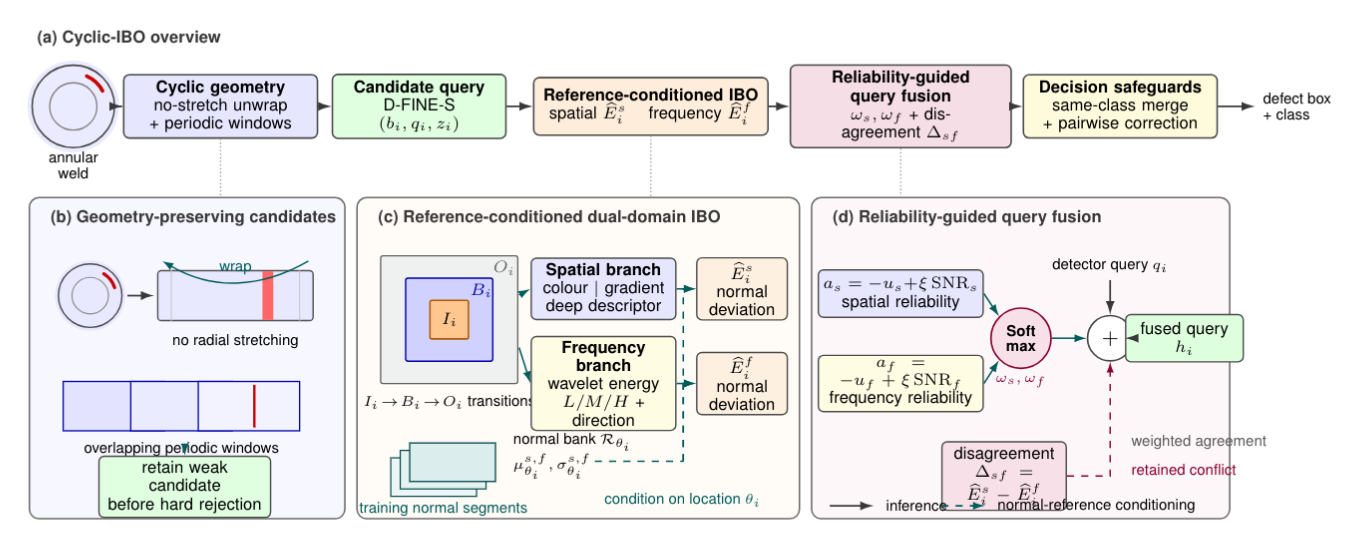
\includegraphics[width=\textwidth]{figures/fig1_cyclic_ibo_overview.png}
\caption{Overview of NORA. (a) The complete candidate--evidence--decision path. (b) No-stretch unwrapping and periodic windows preserve the closed seam while retaining weak detector candidates. (c) Spatial and local-frequency $I\!\rightarrow\!B\!\rightarrow\!O$ transitions are converted into deviations from normal segments at the same circumferential location. (d) Candidate-specific reliability weights combine the two domains while an explicit disagreement path retains diagnostic cross-domain conflict.}
\label{fig:cyclicibo}
\end{figure*}

\subsection{Geometry-Preserving Candidate Queries}

The annular seam band is unwrapped into a strip without radial stretching. It is not resized to force a curved region into a rectangular geometry. The strip is divided into overlapping windows of width 150 pixels. A window that crosses the artificial $0/2\pi$ seam origin is completed with pixels from the opposite end of the strip. This cyclic construction preserves local context for defects near the origin and avoids introducing a nonphysical boundary into the input.

Localization remains the detector's responsibility. NORA operates after a candidate query has been generated because spatial--frequency reasoning cannot recover a defect removed by geometric distortion or missing local context. The centre of candidate $i$ defines a circumferential location bin $\theta_i$. This bin retrieves comparable normal-seam statistics; it is not used as a class label.

\subsection{Normal-Reference IBO Transition Evidence}
\label{sec:ibo-evidence}

\textbf{IBO representation.} Candidate $i$ is decomposed into an interior $I_i$, a scale-adaptive boundary ring $B_i$, and an outside context ring $O_i$. The rings are clipped to the unwrapped seam band. The resulting representation captures two local transitions: from the candidate interior to its boundary and from that boundary to the neighbouring seam.

\textbf{Spatial transition.} From each region $r\in\{I,B,O\}$, we pool colour and luminance statistics $C_{i,r}$ in Lab space, gradient magnitude and orientation $G_{i,r}$, and a deep spatial descriptor $Z_{i,r}$ from the detector feature pyramid:
\begin{equation}
T_{i,r}^{s}=[C_{i,r},G_{i,r},Z_{i,r}].
\end{equation}
The spatial IBO transition is
\begin{equation}
E_i^{s}=[T_{i,B}^{s}-T_{i,I}^{s},\;T_{i,O}^{s}-T_{i,B}^{s}].
\label{eq:spatial-transition}
\end{equation}
It describes local structural change rather than an absolute colour or texture response.

\textbf{Local-frequency transition.} A whole-image Fourier transform does not reliably localize small defects when periodic metal texture dominates the response. We therefore compute a local multi-scale wavelet decomposition independently in $I_i$, $B_i$, and $O_i$. Let $A_{i,r}^{L,M,H}$ denote pooled low-, middle-, and high-frequency energies together with directional responses. The frequency transition is
\begin{equation}
E_i^{f}=[\log A_{i,B}-\log A_{i,I},\;\log A_{i,O}-\log A_{i,B}].
\label{eq:frequency-transition}
\end{equation}
The frequency branch thus evaluates a local spectral transition. It does not assume that greater high-frequency energy always indicates a defect.

\textbf{Normal-reference conditioning.} A reference bank stores $\mathcal R_{\theta}=\{\mu_{\theta}^{s},\sigma_{\theta}^{s},\mu_{\theta}^{f},\sigma_{\theta}^{f}\}$, estimated from verified normal seam segments at each location bin. Both transitions are standardized with the compatible reference:
\begin{equation}
\widehat E_i^d=\frac{E_i^d-\mu_{\theta_i}^d}{\sigma_{\theta_i}^d+\epsilon},\quad d\in\{s,f\}.
\label{eq:reference-conditioning}
\end{equation}
This operation reduces the ambiguity of absolute features. A reflection that routinely occurs at a location can be discounted, whereas a local departure from comparable normal seam remains salient. The candidate under assessment is not used to update its reference entry.

\subsection{Reliability-Guided Spatial--Frequency Query Fusion}
\label{sec:reliability-fusion}

Reliability-guided fusion is the central component of NORA. Fixed concatenation or summation assumes that the two domains are equally dependable. For each $d\in\{s,f\}$, we instead estimate a branch uncertainty $u_d$ and a reference-normalized anomaly strength $\mathrm{SNR}_d$. In the proposed fusion head, a lightweight predictor maps the evidence vector to $u_d\geq0$, and anomaly strength is defined as the normalized evidence magnitude:
\begin{equation}
\mathrm{SNR}_d=\frac{\|\widehat E_i^d\|_2}{\sqrt{\dim(\widehat E_i^d)}}.
\end{equation}
The reliability weights are
\begin{equation}
(\omega_s,\omega_f)=\operatorname{Softmax}(-u_s+\xi\,\mathrm{SNR}_s,\;-u_f+\xi\,\mathrm{SNR}_f),
\label{eq:reliability}
\end{equation}
where $\xi$ controls the contribution of reference-normalized anomaly strength. A branch receives more weight when it is both confident and anomalous relative to normal seam at the same location.

The fused query is
\begin{equation}
h_i=q_i+\omega_sW_s\widehat E_i^s+\omega_fW_f\widehat E_i^f+W_\Delta(\widehat E_i^s-\widehat E_i^f).
\label{eq:fusion}
\end{equation}
The last term does not enforce agreement. It retains diagnostic disagreement patterns. A reflection-like candidate can be spatially strong but spectrally unstable; a small pore can be frequency-dominant at its boundary; and a smoke-like change can be spatially or low-frequency dominant. Accordingly, $h_i$ encodes corroborating evidence and the form of conflict between the two domains. The classification head operates on $h_i$ rather than an unconditioned feature concatenation.

For an end-to-end instantiation, the detector loss is augmented with spatial, frequency, fused-query, and candidate-reliability objectives:
\begin{equation}
\mathcal L=\mathcal L_{\mathrm{D\text{-}FINE}}+\lambda_s\mathcal L_s+\lambda_f\mathcal L_f+\lambda_j\mathcal L_j+\lambda_r\mathcal L_{\mathrm{rel}}.
\label{eq:loss}
\end{equation}
Here, $\mathcal L_{\mathrm{D\text{-}FINE}}$ is the anchor detection objective and its coefficient is fixed to one. The coefficient $\lambda_s$ controls supervision of the spatial-transition branch; it prevents the branch from becoming a passive feature source, but avoids allowing illumination or reflection cues to dominate the detector. Likewise, $\lambda_f$ controls local-frequency supervision, retaining sensitivity to weak boundary and band-transition cues while limiting over-response to metal texture and acquisition noise. The coefficient $\lambda_j$ weights the discriminative objective on the fused query. It requires the combined representation to support the final decision, rather than collapsing to one branch, but does not force spatial and frequency evidence to agree. Finally, $\lambda_r$ weights candidate-reliability supervision. It calibrates the evidence gate so that uncertain or normal-reference-inconsistent evidence cannot dominate the decision; excessive reliability weighting would instead make the detector overly conservative for low-score tail candidates.

The coefficients balance auxiliary evidence learning against detector stability and are selected jointly on the validation set as
\begin{equation}
\max_{\lambda_s,\lambda_f,\lambda_j,\lambda_r,\,k}\; AP_T(k)
\quad\text{s.t.}\quad
AP_H(k)\geq AP_H^{\mathrm{base}}-\delta,
\label{eq:weight-selection}
\end{equation}
where $k$ denotes the checkpoint, $AP_T$ and $AP_H$ denote tail- and head-class AP, and $\delta$ is the permitted head-class reduction. This criterion selects evidence weights and a checkpoint for tail improvement without accepting an unconstrained loss of head-class performance.

\subsection{Decision Safeguards: Cyclic Merging and Restricted Correction}

Overlapping cyclic windows can generate several hypotheses for one physical defect. We merge only boxes with the \emph{same predicted class} across overlapping windows. No cross-class vote is permitted. This removes duplicate predictions without enabling a frequent class to absorb a weak tail class during merging.

A second global classifier would create additional opportunities for error across the full label space. We instead construct a confusion graph from held-out error audits and activate contrastive correction only for recurrent tail-to-head or visually similar pairs. Within an active pair, the candidate crop and fused query $h_i$ are compared with pair-specific prototypes. The correction may re-rank the pair but cannot propose a class outside the audited pair. This restricts the operation to observed confusions while preserving the detector's original decision space.

\section{Experimental Setup}

\subsection{Industrial Dataset and Long-Tail Protocol}

The in-house annular-weld dataset contains 22 raw annotated defect classes, with 4,700 training and 1,124 validation instances. For the class-grouped evidence audit, small smoke, smoke cluster, and smoke are merged; missing weld, long weld-height collapse, missing-weld blue-black, and seam blue-black are merged. Steel cap, pad separation, missing-weld crack, desoldering, and weld-height seam are excluded. This produces the 1,122-instance evaluation scope in Table~\ref{tab:dataset}. The distribution remains strongly imbalanced: the largest class has 259 validation instances, whereas pit has two. We additionally audit six rare and operationally important focus-tail defects, comprising 33 validation instances. For this subset, we report correct, wrong-class, and missed detections explicitly. A tail gain is not meaningful if missed instances are merely replaced by incorrect class assignments.

\begin{table}[t]
\caption{Class-grouped industrial validation protocol after the specified merges and exclusions. The raw train/validation splits contain 4,700/1,124 instances; the evidence audit uses the 1,122 effective validation instances below.}
\label{tab:dataset}
\centering
\scriptsize
\setlength{\tabcolsep}{2.6pt}
\begin{tabular}{llr}
\toprule
Frequency group & Class after merging & Val. instances \\
\midrule
Head & Weld-height stripe & 259 \\
     & Smoke family & 204 \\
     & Missing-weld/collapse family & 232 \\
\midrule
Medium & Weld hole / long height crack & 79 / 69 \\
       & Weld explosion / high smoke & 62 / 76 \\
\midrule
Tail & Long weld hole / point height & 71 / 37 \\
     & Slag / gray weld / pit & 22 / 9 / 2 \\
     & Long weld height & 0 \\
\midrule
\textbf{Total} & \textbf{13 grouped classes} & \textbf{1,122} \\
\bottomrule
\end{tabular}
\end{table}
\subsection{Implementation and Fusion Ablation}

D-FINE-S with an HGNetv2-B0 backbone serves as the candidate generator. The in-house detector is trained for 32 epochs, and the epoch-14 checkpoint is selected. The annular strip is processed using no-stretch, periodic overlapping windows in the 150-pixel seam-height configuration. Candidate-generation controls compare direct circular input, ordinary unwrapping, extended-context unwrapping, and periodic 150-pixel windows.

The completed industrial evidence ablation compares A0, D-FINE score; A1, $+$ IBO spatial/group evidence; A2, $+$ normal-reference distance; A3, $+$ local-frequency evidence; A4, $+$ normal-reference and frequency evidence; and A5, $+$ restricted gray-weld versus collapse-family correction. Each variant uses the same candidate groups and class-merging protocol, with its operating threshold selected from the predefined sweep. This A0--A5 study tests the implemented post-detection evidence pipeline and reports both all-class and focus-tail outcomes. It is distinct from a future end-to-end query-head ablation of fixed fusion, normal-reference conditioning, reliability weighting, and disagreement modeling.

\noindent\textbf{Eligibility of additional long-tail comparators.} The primary in-house comparison includes methods whose final predictions have been re-audited with the same 1,122-instance grouping, matching rule, and correct/wrong-class/missed accounting. The three-stage SimLTD-style D-FINE-S schedule is included because its final stage has passed this identical audit. It retains the D-FINE-S architecture and applies a 20/6/6 head--tail--joint schedule; it is therefore reported as a \emph{SimLTD-style adaptation}, rather than as an official reproduction of SimLTD. The ROG Faster R-CNN R50FPN transfer model has also passed the same audit at $t=.25$ and is included as an architecture-diverse comparator. FRACAL is included with a dagger as a budget-matched calibration audit: its multiplicative post-calibration score uses a different operating scale and a separately frozen D-FINE-S candidate generator. Its overall, gray-weld, and collapse-family audit values are reported, while the unavailable identical focus-tail aggregate is marked ``--'' rather than inferred.
\subsection{LVIS Transfer Pilot}

We also use a pilot split of the LVIS long-tailed benchmark~\cite{gupta2019lvis}. The split comprises 10,000 training images with 117,605 annotations and 2,000 validation images with 20,891 annotations across 1,203 mapped categories. D-FINE-S is trained for 100 epochs using 640-pixel no-stretch resizing. Annular ROI extraction, unwrapping, and cyclic windows are disabled. IBO candidates are extracted at score 0.25. The normal-reference evidence model uses 12,000 normal samples, $k=5$ neighbours, a 256-pixel feature side, and seed 0. This transfer experiment evaluates candidate reliability rather than a replacement detector head. AUROC, AUPR, and $(C,W,M)$ under a common candidate-projection protocol are therefore its primary outcomes. We additionally export official LVIS AP as a secondary alignment check. For method-level context, we run FRACAL as an inference-only, per-image budget-matched recalibration of the frozen D-FINE-S outputs, and run the public SimLTD codebase with a 20/6/6 staged fast-pilot schedule. The latter uses the same split and 640-pixel preprocessing but is explicitly not the full official SimLTD training schedule.

\subsection{Metrics}

We report standard detector measures---AP, AP50, AP75, precision, and recall---whenever they are defined by the benchmark protocol. The industrial validation also records $(C,W,M)$, the numbers of correct, wrong-class, and missed instances. The class-aware matched rate is $C/N$, where $N$ is the number of annotated instances. Candidate coverage, tail-to-head confusion counts, and focus-tail outcomes are reported alongside aggregate metrics. This protocol distinguishes a reduction in missed tail defects from a recall gain caused by additional wrong-class selections.

\textbf{Benchmark-aligned long-tail reporting.} The following benchmark-specific comparisons use fixed evaluation protocols. For the LVIS pilot and the SimLTD fast-pilot implementation~\cite{tran2025simltd}, we use the official LVIS API and report box AP together with AP50, AP75, and the frequency-group measures APr, APc, and APf. These are the average precisions for rare, common, and frequent LVIS categories, respectively; AR@300 is reported as a recall-oriented secondary measure. Candidate-level $(C,W,M)$, AUROC, AUPR, and $C/N$ are diagnostic measures; they must not be presented as substitutes for official LVIS AP. The corresponding numerical comparisons are reported separately for each benchmark, rather than mixing non-equivalent metrics in one table.

\section{Results and Discussion}

\subsection{Geometry-Preserving Candidate Generation}

Table~\ref{tab:geometry} quantifies candidate generation before any IBO evidence is computed. Direct circular input achieved a class-aware matched rate of 76.87\%. Ordinary unwrapping increased the rate to 79.45\%, whereas extended context alone did not improve the result. Periodic 150-pixel windows achieved 85.77\% and reduced misses from 207 to 88. These results show that the geometry-preserving front end improves candidate availability. They do not, by themselves, demonstrate the contribution of spatial--frequency fusion.

\begin{table}[t]
\caption{Candidate-generation comparison on the 1,124-instance validation set. $C$, $W$, and $M$ denote correct, wrong-class, and missed instances.}
\label{tab:geometry}
\centering
\small
\begin{tabular}{lrrrr}
\toprule
Setting & $C$ & $W$ & $M$ & $C/N$ (\%) \\
\midrule
Circular input & 864 & 53 & 207 & 76.87 \\
Ordinary unwrap & 893 & 63 & 168 & 79.45 \\
Extended context & 884 & 54 & 186 & 78.65 \\
Periodic 150 px & \textbf{964} & 72 & \textbf{88} & \textbf{85.77} \\
\bottomrule
\end{tabular}
\end{table}

\subsection{Industrial Candidate Reliability and Error Trade-off}

Table~\ref{tab:ibo-reliability} reports the completed A0--A5 post-detection evidence ablation. All variants use the same D-FINE candidate groups and class-merging protocol; the operating threshold $t$ is selected separately from each variant's predefined sweep. A0 uses the detector score alone. A1 introduces IBO spatial/group evidence, A2 additionally uses the normal-reference distance, A3 uses local-frequency evidence, A4 combines normal-reference and frequency evidence, and A5 applies restricted gray-versus-collapse confusion-pair correction after A4.

The all-class matched rate changes only slightly from A0 to A4. The principal long-tail effect appears in A5: the focus-tail matched rate rises from 81.56\% to 83.69\%, and gray-weld detection rises from $5/9$ to $8/9$. The explicit collapse-family column exposes the cost of this correction: its matched rate falls from 98.28\% to 94.40\%. Accordingly, all-class $C/N$ decreases by 0.62 points, from 93.67\% to 93.05\%, because a small number of collapse-family instances are reassigned. The result therefore supports the intended interpretation: confusion-pair correction is a targeted tail-recovery mechanism, not an unconditional replacement for the base decision. Figure~\ref{fig:real-corrections} shows two corresponding validation cases: the same local candidate is labeled as gray weld, assigned to the collapse family by D-FINE, and then re-ranked to gray weld by the restricted NORA correction.

\begin{table}[t]
\caption{Completed A0--A5 post-detection evidence ablation on 1,122 class-grouped validation instances. $t$ is selected from the predefined sweep. Tail and collapse entries are $C/N$ (\%); gray-weld entries are $C/W/M$.}
\label{tab:ibo-reliability}
\centering
\scriptsize
\setlength{\tabcolsep}{2.0pt}
\begin{tabular}{clcrrrc}
\toprule
Var. & Evidence added & $t$ & All & Tail & Collapse & Gray \\
\midrule
A0 & D-FINE score & .25 & \textbf{93.67} & 81.56 & \textbf{98.28} & 5/4/0 \\
A1 & + IBO spatial/group & .30 & 93.49 & 80.85 & \textbf{98.28} & 5/4/0 \\
A2 & + normal reference & .35 & 93.49 & 80.85 & \textbf{98.28} & 5/4/0 \\
A3 & + local frequency & .10 & 93.58 & 81.56 & \textbf{98.28} & 5/4/0 \\
A4 & + normal reference + frequency & .15 & 93.58 & 81.56 & \textbf{98.28} & 5/4/0 \\
A5 & + restricted confusion correction & .15 & 93.05 & \textbf{83.69} & 94.40 & \textbf{8/1/0} \\
\bottomrule
\end{tabular}
\end{table}
\begin{table*}[!t]
\caption{Primary in-house comparison under the 1,122-instance class-grouped audit. All methods use no-stretch periodic 150-pixel seam strips. D-FINE-S, SimLTD-style, and NORA share the D-FINE-S detector, whereas ROG uses its Faster R-CNN implementation. FRACAL$^{\dagger}$ is a budget-matched calibration of a separately frozen D-FINE-S candidate generator at $t=.056$, rather than a matched-decision detector run; its source audit does not contain the identical focus-tail aggregate, hence ``--''. $C/W/M$ reports correct, wrong-class, and missed instances. Tail and collapse values are matched rate $C/N$ (\%); gray-weld is $(C/W/M)$.}
\label{tab:inhouse-comparison}
\centering
\small
\setlength{\tabcolsep}{4.0pt}
\begin{tabular}{lllrrrrr}
\toprule
Method & Decision setting & Input & $C/W/M$ & All $C/N$ & Tail $C/N$ & Gray & Collapse $C/N$ \\
\midrule
D-FINE-S & detector score, $t=.25$ & periodic 150-px strip & 1051/44/27 & \textbf{93.67} & 81.56 & 5/4/0 & \textbf{98.28} \\
SimLTD-style & 20/6/6 head--tail--joint schedule, $t=.25$ & periodic 150-px strip & 1028/57/37 & 91.62 & 80.85 & 0/8/1 & 91.81 \\
ROG & Faster R-CNN R50FPN transfer, $t=.25$ & periodic 150-px strip & 948/71/103 & 84.49 & 74.47 & 0/1/8 & 83.62 \\
FRACAL$^{\dagger}$ & budget-matched calibration, $t=.056$ & periodic 150-px strip & 931/147/44 & 82.98 & -- & 3/6/0 & 93.53 \\
NORA (A4) & IBO + normal reference + frequency, $t=.15$ & periodic 150-px strip & 1050/45/27 & 93.58 & 81.56 & 5/4/0 & \textbf{98.28} \\
NORA (A5) & A4 + restricted confusion correction, $t=.15$ & periodic 150-px strip & 1044/51/27 & 93.05 & \textbf{83.69} & \textbf{8/1/0} & 94.40 \\
\bottomrule
\end{tabular}
\end{table*}
\begin{figure*}[t]
\centering
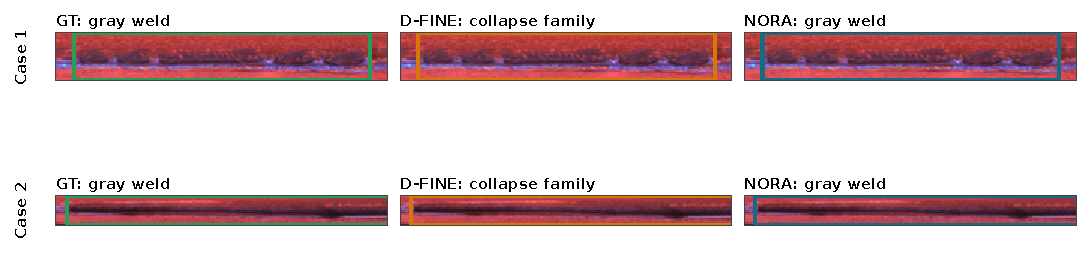
\includegraphics[width=\textwidth]{figures/fig2_real_nora_corrections.pdf}
\caption{Two real validation cases corrected by the restricted gray-weld versus collapse-family module. Each row shows the same no-stretch weld-strip crop. D-FINE assigns the candidate to the collapse family, whereas NORA re-ranks it as gray weld, matching the annotation. These examples visualize the targeted tail recovery quantified in Table~\ref{tab:ibo-reliability}; they do not imply that every collapse-family prediction should be changed.}
\label{fig:real-corrections}
\end{figure*}
\subsection{LVIS Pilot: Transfer of Candidate Reliability}
\label{sec:lvis-results}

The LVIS pilot evaluates normal-reference evidence outside annular-weld geometry. On 33,006 validation candidates, the reliability model achieved AUROC $=0.6890$, AUPR $=0.5275$, and Brier score $=0.2511$. Table~\ref{tab:lvispilot} reports the official-LVIS API results; candidate recovery is reported in the accompanying thresholded-projection audit. Relative to the D-FINE score threshold of 0.40, reliability threshold 0.15 retained more candidates, increased correctly covered instances by 1,945, and reduced misses by 3,990. It also increased wrong-class instances by 2,045. The 9.31-point gain in $C/N$ is therefore a recall-oriented candidate-recovery result, not a free improvement in final classification.

\begin{table*}[!t]
\caption{LVIS pilot method comparison under the official LVIS API. AP, AP50, AP75, APr, APc, and APf are percentage metrics. All methods use the same 10k/2k pilot split and 640-pixel no-stretch input. D-FINE-S and NORA share the frozen 100-epoch D-FINE-S candidate generator; FRACAL recalibrates its outputs with an equal per-image prediction budget; ROG is an independently trained Faster R-CNN R50FPN transfer model run for 32 epochs; and SimLTD uses its public codebase with a 20/6/6 fast-pilot schedule, not the full official schedule. Candidate-level $C/N$ is discussed separately because it uses a thresholded projection audit rather than the full prediction ranking.}
\label{tab:lvispilot}
\centering
\scriptsize
\setlength{\tabcolsep}{3.2pt}
\begin{tabular}{lllrrrrrr}
\toprule
Method & Learning setting & Input & AP & AP50 & AP75 & APr & APc & APf \\
\midrule
D-FINE-S & raw candidate ranking & 640, no stretch & 8.008 & 11.869 & 8.218 & 0 & 2.096 & 12.165 \\
FRACAL & inference-only, budget-matched recalibration & 640, no stretch & 8.457 & 12.583 & 8.588 & .223 & 2.584 & 12.612 \\
ROG & Faster R-CNN R50FPN transfer, epoch 32 & 640, no stretch & 10.800 & 21.200 & 9.800 & 2.400 & 9.400 & 12.300 \\
SimLTD & public codebase, 20/6/6 fast pilot & 640, no stretch & \textbf{12.700} & \textbf{20.600} & \textbf{12.900} & \textbf{6.600} & \textbf{11.300} & \textbf{14.100} \\
NORA & IBO reliability, $t=.15$ & 640, no stretch & 8.008 & 11.869 & 8.218 & 0 & 2.096 & 12.165 \\
NORA & reliability + restricted correction & 640, no stretch & 8.008 & 11.869 & 8.218 & 0 & 2.096 & 12.165 \\
\bottomrule
\end{tabular}
\end{table*}

The local query corrector used 15 confusion-cluster models derived from 30 training-only confusion edges. At probability/margin gates $(0.55,0.15)$, it re-ranked 2 of 33,006 validation candidates. At $(0.65,0.20)$, it re-ranked none. The corresponding $(C,W,M)$ summaries were unchanged. The restriction avoids broad label-space changes, but it is too conservative to demonstrate an aggregate gain in this pilot.

For benchmark alignment, we additionally exported the frozen candidate outputs to the official LVIS API. The raw candidate set obtained AP $=8.008\%$, AP50 $=11.869\%$, AP75 $=8.218\%$, APr $=0$, APc $=2.096\%$, and APf $=12.165\%$. FRACAL's budget-matched recalibration raised AP to $8.457\%$. The completed SimLTD fast pilot reached AP $=12.700\%$, AP50 $=20.600\%$, AP75 $=12.900\%$, APr $=6.600\%$, APc $=11.300\%$, and APf $=14.100\%$. This SimLTD row uses the public codebase and the official LVIS evaluator, but its shortened 20/6/6 schedule is not a full official-schedule reproduction. Reliability filtering and the restricted corrector changed NORA's AP by less than $0.001$ percentage points. Thus, the present pilot supports candidate-level recovery but does \emph{not} demonstrate an official LVIS AP gain; this distinction is maintained by reporting official AP separately from the candidate-projection audit.

\subsection{Scope of the Fusion Claim}

The completed industrial and LVIS studies support three narrower findings. Cyclic geometry improves candidate availability. Normal-reference evidence can retain low-score candidates. Conservative local correction does not produce measurable global degradation in this pilot. The studies do not yet establish that the learned query-level fusion in Section~\ref{sec:reliability-fusion} outperforms fixed spatial--frequency concatenation. That claim requires the B0--B6 comparison specified in Section~3, particularly B3 (fixed fusion), B4 (normal-reference conditioning), and B5 (reliability plus disagreement). Stating this boundary prevents candidate-stage improvements from being interpreted as an end-to-end detector gain.

\section{Conclusion}

NORA formulates long-tailed annular weld inspection as a query-level evidence-reliability problem rather than a score-thresholding problem. Its central design combines normal-reference IBO transitions in the spatial and local-frequency domains using candidate-specific reliability. The disagreement between domains is retained as evidence instead of being removed by a fixed feature mixture. On the industrial data, geometry preservation improved candidate availability and evidence-based re-evaluation reduced misses. The LVIS pilot showed that normal-reference reliability transfers at the candidate level. The conservative confusion corrector left aggregate LVIS instance statistics unchanged, which defines its present limitation. A completed B0--B6 end-to-end fusion ablation and an official LVIS AP evaluation are still required before claiming that the proposed fusion outperforms conventional spatial--frequency fusion. Subsequent validation should also assess reference-bank updates across acquisition conditions and the runtime cost of joint fusion in production inspection.


\clearpage
\raggedbottom
\bibliographystyle{IEEEbib}
\bibliography{refs}

\end{document}
